% Preamble:
% \usepackage{tikz}
% \usepackage{subcaption}

\begin{figure}[ht]
\centering

\begin{subfigure}[t]{0.22\textwidth}
\centering
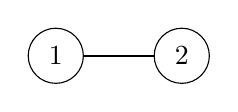
\begin{tikzpicture}[v/.style={circle,draw,minimum size=7mm}, e/.style={thick}]
\node[v] (1) at (0,0) {1};
\node[v] (2) at (1.6,0) {2};
\draw[e] (1)--(2);
\end{tikzpicture}
\caption{$K_2$}
\end{subfigure}
\hfill
\begin{subfigure}[t]{0.22\textwidth}
\centering
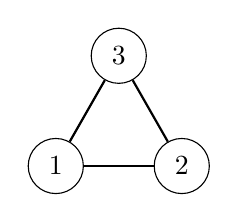
\begin{tikzpicture}[v/.style={circle,draw,minimum size=7mm}, e/.style={thick}]
\node[v] (1) at (0,0) {1};
\node[v] (2) at (1.6,0) {2};
\node[v] (3) at (0.8,1.4) {3};
\draw[e] (1)--(2);
\draw[e] (2)--(3);
\draw[e] (3)--(1);
\end{tikzpicture}
\caption{$K_3$}
\end{subfigure}
\hfill
\begin{subfigure}[t]{0.22\textwidth}
\centering
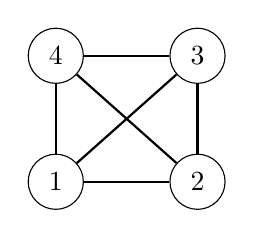
\begin{tikzpicture}[v/.style={circle,draw,minimum size=7mm}, e/.style={thick}]
\node[v] (1) at (0,0) {1};
\node[v] (2) at (1.8,0) {2};
\node[v] (3) at (1.8,1.6) {3};
\node[v] (4) at (0,1.6) {4};
\draw[e] (1)--(2);
\draw[e] (2)--(3);
\draw[e] (3)--(4);
\draw[e] (4)--(1);
\draw[e] (1)--(3);
\draw[e] (2)--(4);
\end{tikzpicture}
\caption{$K_4$}
\end{subfigure}
\hfill
\begin{subfigure}[t]{0.22\textwidth}
\centering
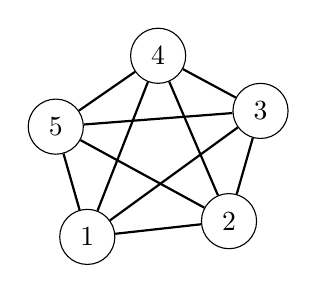
\begin{tikzpicture}[v/.style={circle,draw,minimum size=7mm}, e/.style={thick}]
\node[v] (1) at (0,0) {1};
\node[v] (2) at (1.8,0.2) {2};
\node[v] (3) at (2.2,1.6) {3};
\node[v] (4) at (0.9,2.3) {4};
\node[v] (5) at (-0.4,1.4) {5};
\draw[e] (1)--(2);
\draw[e] (1)--(3);
\draw[e] (1)--(4);
\draw[e] (1)--(5);
\draw[e] (2)--(3);
\draw[e] (2)--(4);
\draw[e] (2)--(5);
\draw[e] (3)--(4);
\draw[e] (3)--(5);
\draw[e] (4)--(5);
\end{tikzpicture}
\caption{$K_5$}
\end{subfigure}

\caption{Complete graphs $K_n$ for $n=2,3,4,5$.}
\label{fig:complete-k2-k5}
\end{figure}
